\section{TRI-D Interferometric imaging}\seclab{Intf}

Interferometry can be performed working only with the signals measured in the antennas, i.e.\ without unfolding the antenna function, and is referred to as Signal Interferometry (SI), which is by now considered obsolete. This because the method has many unsolved issues with signs due to the antenna function and the emission pattern being angle dependent. More sophisticated is to convert the measured signal in the X- and Y- dipoles to the radiation electric field at the antenna and use this for interferometry, presently the preferred and only option. This will be named E-field Interferometry (EI) when it needs to be contrasted with SI.

Source finding is performed by the script \verb!"Interferometry.sh"! residing in the FlashFolder. The running of the script is controlled by \verb!"Interferometry.in"!, which typically resembles:

\begin{linenumbers}
\resetlinenumber
\begin{verbatim}
 &Parameters  RunOption= "TRI-D"
! CurtainHalfWidth= 100     ! Produce a "Curtain" plot when positive.
! Simulation= ""     ! Run on simulated data from such files.
 ChainRun= 0     ! Automatically start jobs (for - previous or + following timeslots, made to follow a negative leader.
 IntfSmoothWin= 19     ! Width (in samples) of the slices for TRI-D imaging.
! PixPowOpt= 0     ! =0=default: Intensity=sum two transverse polarizations only; =1: Intensity=sum all polarizations weighted with alpha == intensity of F vector; =2: Intensity=sum all three polarizations, including longitudinal with the full weight
 TimeBase=320    ! Time-offset from the start of the data, best if kept the same for all analyses for this flash
 NoiseLevel= 1.0000000000000000E-002     ! Any weaker sources will not be imaged.
 CalibratedOnly= T     ! Use only antennas that have been calibrated.
 AntennaRange= 100.     ! Maximum distance (from the core) for the range of the antennas (in [km]).
 SaturatedSamplesMax= 3     ! Maximum number of saturates time-samples per chunk of data
 Calibrations="Calibrations202202071332.dat" ! FldCal all antennas
 BadAnt_SAI=   5095,   7093,  11089,  13088,  13089,  17084,  17085,  17094,  17095
               101085, 141083, 141086, 141087, 167094, 169082, 169090, 169094,
 ExcludedStat=  "RS305"      ! Mnemonics of the stations that should be excluded.
 SignFlp_SAI=  142092, 142093
 OutFileLabel= "XYZ"
 &end  !
S    8.2 ,-3.7, -34.11    !    Reference/Source-| time, & position
C   80 2.5, 30 2.5, 72 4 !   Polar(Phi,Th,R)/Carthesian(N,E,h) | 3x(grid spacing, #gridpoints)
F  25000  15000 10.   !  First/Median| SumStrt, SumWindw, AmpltPlot
\end{verbatim}
\end{linenumbers}

*** Obviously more editing needed, not up-to-date yet ******

The lines in the namelist \verb!"&Parameters"! input specify:
\begin{enumerate*}
\item[1] \verb!'RunOption= "TRI-D"'!: Run the TRI-D Imager
\item[2] \verb#"! CurtainHalfWidth= 100"#: Produce "Curtain" plots when positive.
\item[3] \verb#"IntfPhaseCheck=.false."#: Do not print for each antenna the amplitude, phase, and angle to the source, done for the central pixel. This can be helpful to check if there are certain stations that are off in certain ways, but the info is difficult to interpret. Make sure that the direction for the central pixel is such that it is perfect for the largest source in the selected time trace. When commented, this information will appear in the output.
\item[4] \verb!"! CurtainPlot=.true."!: When un-commented, a curtain plot (see \secref{Curtainplot}) will be made for the time-traces lined up for the central pixel.
\item[5] \verb!"TimeBase=669."!: This time is added to the relative time specified in the input.
\item[6] \verb!"Calibrations ="!: The name of the file containing calibration and RFI information.
\item[7] \verb!"BadAnt_SAI="!: These antennas are excluded from the analysis.
\item[10] \verb!"SignFlp_SAI="!: The amplitude for this antenna is multiplied by minus unity.
\item[11] \verb!"ExcludedStat="!: Mnemonics of the stations that will be excluded from interferometry. The exclusion is usually based on unexpected phases seen when running with \verb!"IntfPhaseCheck=.true."!.
\item[12] \verb!"OutFileLabel="!: Additional label used for the output files, including the plots.
\item[13] \verb!"AntennaRange="!: The maximal distance (in [km]) from the reference station of the antenna stations that are included in interferometry.
\item[14] \verb!"IntfSmoothWin="!: Integer. The width of the sampling function used for Time Resolved Imaging (in [samples]). This number should be of the order of the impulse-response time, about 20~samples.
\item[15] \verb!"Dual="!: default=.true. in version 20 and higher. Include antenna function and unfold polarization in interference calculation and use the approach discussed in \secref{E_Intf}.
   \\ \verb!"Dual=.false."!: Perform the interferometry separately for the X- and Y-LOFAR dipoles (the odd and even antennas).
\item[16] \verb!"PixPowOpt="!: Integer. Selects how the intensity of a pixel is calculated.
   \\\verb!PixPowOpt =0! (default): sum two transverse (as seen from the core) polarizations only.
   \\\verb!PixPowOpt =1! : sum all polarizations weighted with alpha to compensate $A^{-1}$ thus intensity =  $|\vec{F}|$, see \eqref{F_as}.
   \\\verb!PixPowOpt =2! : Sum all three polarizations, thus including longitudinal with the full weight.
\item[17] \verb!"ChainRun="!: Integer. If =0 the present run will not spawn any children. \\If positive another run is generated with identical parameters except
     \begin{itemize}
     \item The central location of the hypercube (line 17) which will be pinned down to the most intense spot for the present time interval.
     \item The start time (line 17) will be increased by 0.3~ms. If the total window (line 19) equals 60040 (line 19, where 40=$2\times$"IntfSmoothWin") this will generate image data that can later be stitched together to generate (using \secref{InterfSrcSel}) a continuous image along a negative leader.
     \item The absolute value of \verb!"ChainRun"! is decreased by unity.
     \item The present value of \verb!"ChainRun"! is worked into \verb!"OutFileLabel"! as well as the naming of the spawned scripts.
     \end{itemize}
     If "ChainRun=" negative, the same will be done, only backward in time. \\Chaining jobs works only on Linux systems.
\item[18] \verb!"NoiseLevel="!: Only sources with a coherent intensity exceeding this will be imaged.
\end{enumerate*}

The following lines specify:
\begin{description}
\item[245.1 , $\cdots$]
   Entry\#1) Starting time in the trace (in the reference antenna, which differs from the time of the sources) of the data-chunk that will be used. Time is taken relative to \verb!"TimeBase"!.
   \\Entry\#2-4) Coordinates of the central pixel in (N,E,h) notation. The units may be [km].
\item[P  50 .005, $\cdots$]
   Entry\#1) If capital "P" or "C" a Polar or Cartesian grid is forced. If anything else (including a space) a reasonable choice is made based on the specified grid structure. A Polar grid (recommended) is specified in the order: Azimuth angle $\phi$, elevation angle $\theta_e$, distance to reference antenna $R$. A Cartesian grid as: Northing $N$, Easting $E$, altitude $h$. Internally both are used in parallel.
   \\Entry\#2, 4, 6) Number of grid points.
   \\Entry\#3, 5, 7) Grid spacing.
\item[4000  $\cdots$]
   Entry\#1) The first sample number used for interferometric imaging of the trace. The program needs select some previous channels as a buffer to be able to image the indicated part of the chunk in the reference antenna. The first sample thus be larger than zero. Error messages are generated and image is truncated when the value is too small.
   \\Entry\#2) The length of the window (in [samples]) used for imaging. 60k~samples corresponds to 0.3~ms. The additional 40 (=$2\times$"IntfSmoothWin") is to accommodate for the beginning and end smoothing windows when performing Time Resolved Imaging (see \secref{TRID}).
\end{description}


This script produces interferometric images (see \secref{TRID} for the procedures followed)
and puts the results in several data files in the subdirectory \verb!"files"!. It also prepares the command files (in \verb!"GLE-plotsXYZ.sh"!) for running the GLE scripts \cite{GLE} to produce \verb!"InterfContourXYZ.pdf"!, \verb!"XYZInfImgBar_0.pdf"!, \verb!"XYZInfImaMx_0.pdf"!, \verb!"InterfTrackXYZ.pdf"!. The interferometric hypercube is also shown in the plot of the source locations.

It is recommended to subsequently run the script \verb!"InterfSrcSel.sh"! using \verb!"InterfSrcSel.in"! as input to produce the plots that are zoomed in on the region of interest, see \secref{InterfSrcSel}.

\subsection{Output}\seclab{Interf}

The produced .dat files are plain text files and contain some header lines with some general information followed by the specific data of the sources that are found and pass some very crude criteria. The files have a format that is suitable for the plotting script \verb!"SourcesPlot.gle"!. The naming of these data files is as in \verb!"XYZIntfSpecPowMx_d.dat"!, where \verb!"XYZ"! is set by the user through \verb!"OutFileLabel=XYZ"! when running the interferometry option; \verb!"IntfSpecPow"! is fixed for these kind of files; \verb!"Mx"! implies that these source positions were determined using the quadratic maximum search while for \verb!"Bar"! the, by now obsolete, barycentric procedure was used, see \secref{Max}.
This file also contains the coordinates of the corners of the hypercube used in the interferometry calculation.


\subsubsection{Intensity plot}

\begin{figure}[th]
\centering{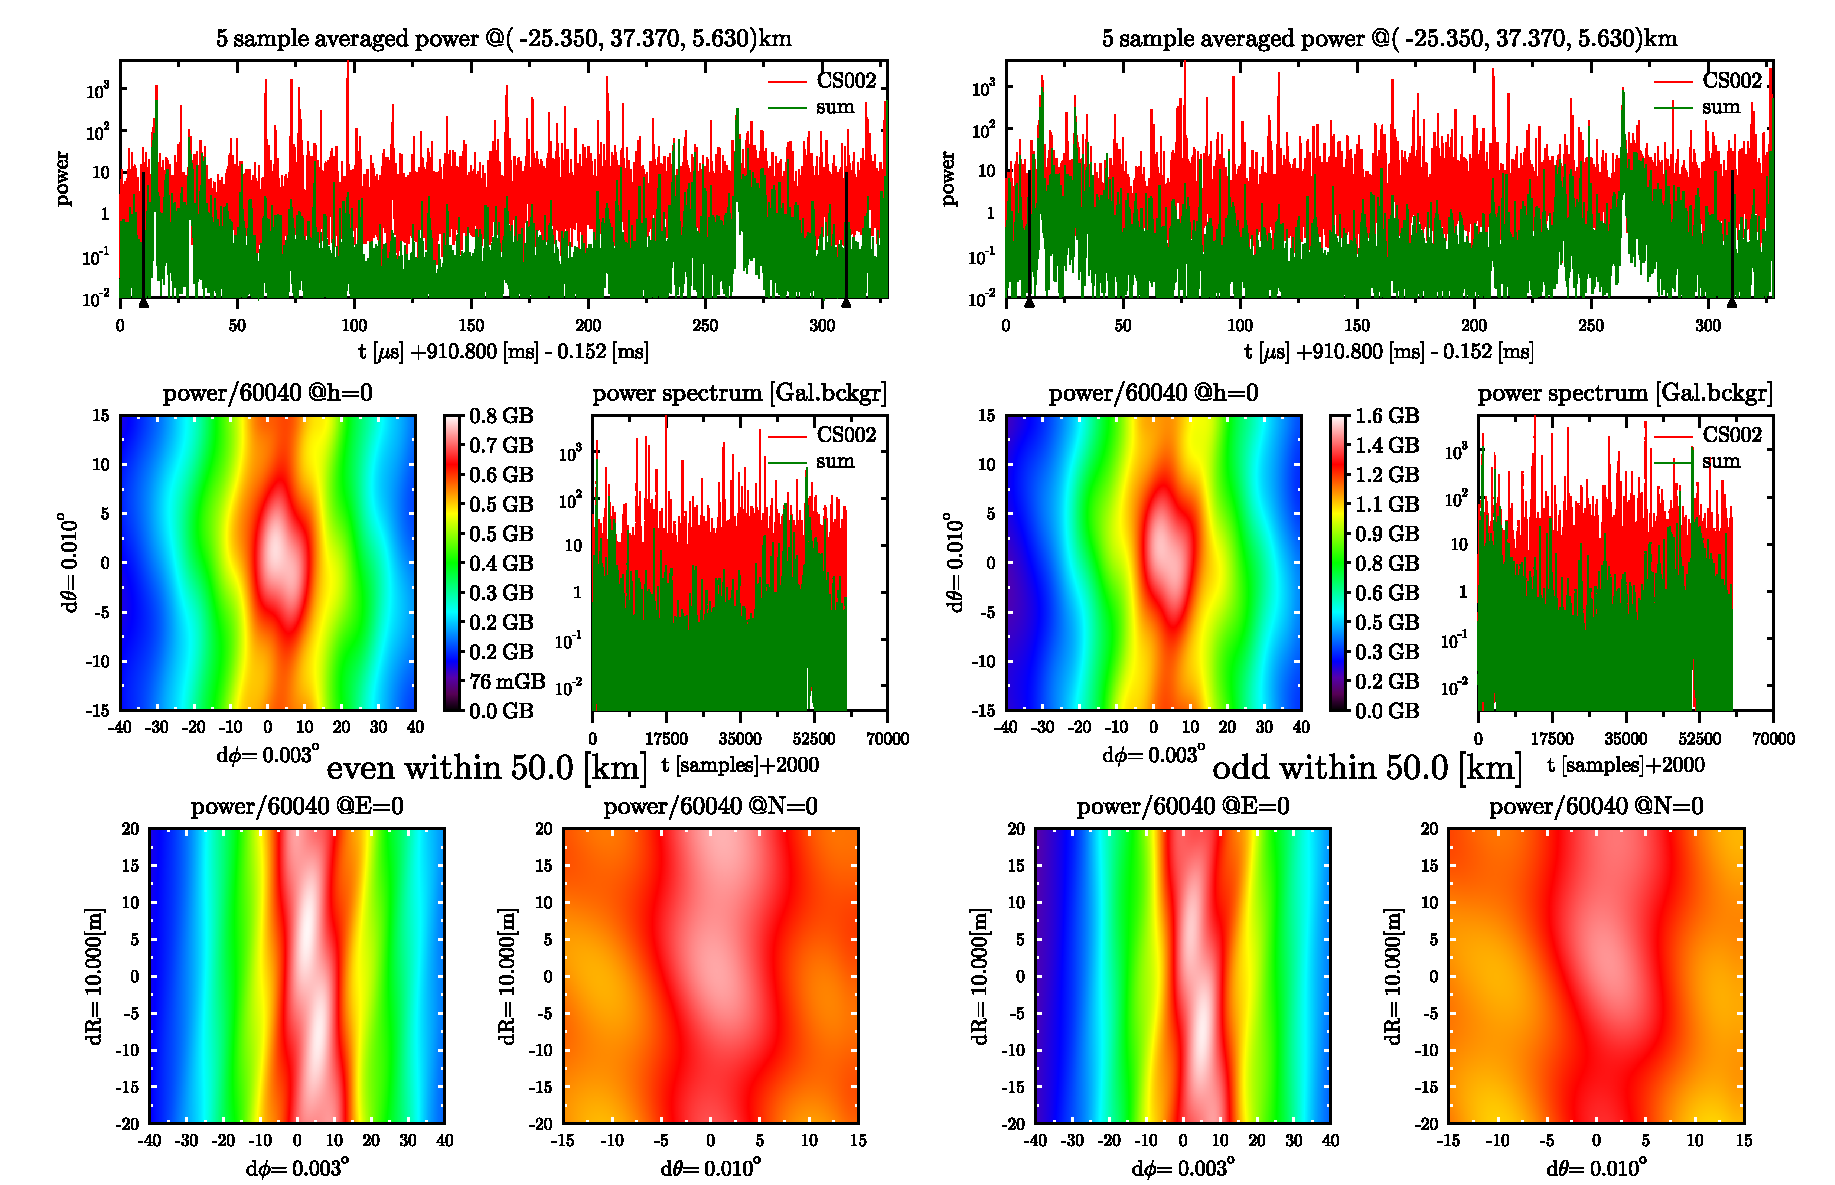
\includegraphics[width=0.99\textwidth]{Figs/InterfContourSE20A7-Np-} }
%\centering{\includegraphics[ bb=1.0cm 2.4cm 24.5cm 25.7cm,clip, width=0.49\textwidth]{../Figs/SE20A7-NPMx_1HIntfSpecSel} }
	\caption{Typical image for the TRID Imager as created by running ``InterfSrcSel.sh".}	 \figlab{TRIDIntImg}
\end{figure}

A typical interferometric Intensity plot is shown in \figref{TRIDIntImg}. These are produced separately for even- (left side of \figref{TRIDIntImg}) and odd- (right side) numbered antennas. The top shows in red the spectrum in the reference antenna while green shows the coherent sum of all antennas in the field, beamed towards the central pixel of the hypercube. The green spectrum is normalized by the number of antennas ($N_a$, i.e.\ the geen and red should fall on top of each other if the signal would be completely coherent for this direction. If the signal is random noise it should be at a fraction of 1/$N_a$. This signal power is rebinned over 5 samples. With black lines the zoom-in window is indicated. The zoomed-in spectrum is shown below it, using the same convention but without re-sampling. The other figures show the intensity along a plane through the hypercube, top left at dR=0, the bottom two at $d\theta=0$ and $d\phi=0$. Step sizes and ranges are specified in the input line starting with `P'.

\begin{figure}[th]
\centering{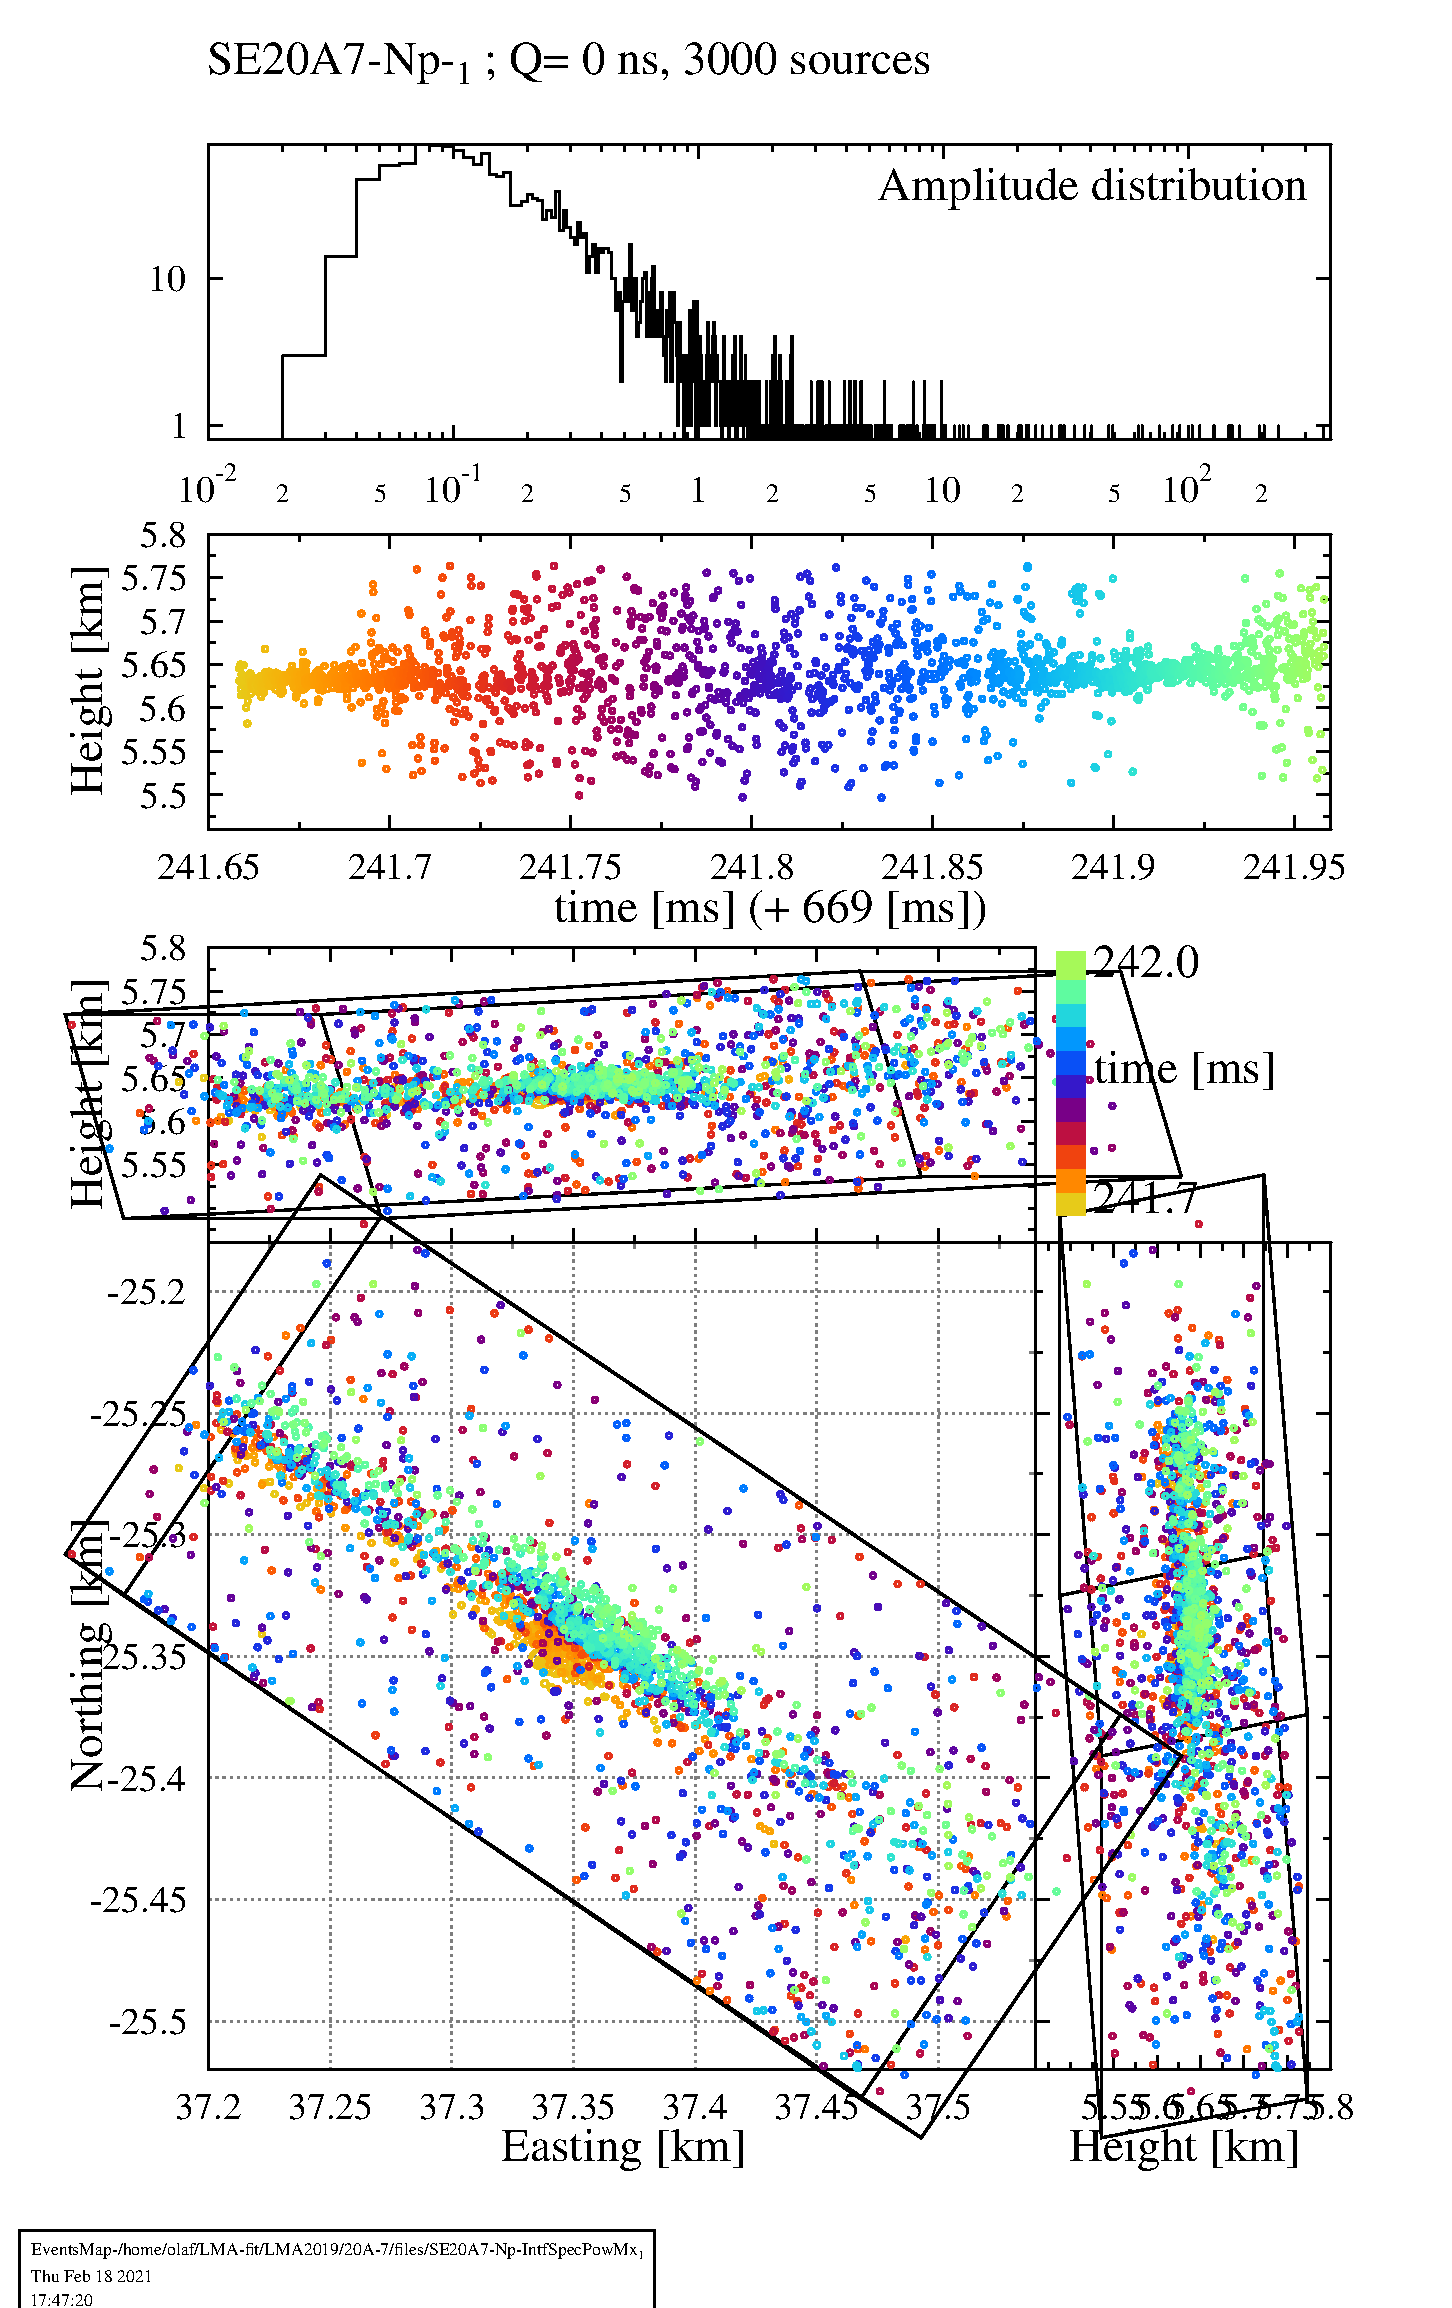
\includegraphics[width=0.49\textwidth]{Figs/SE20A7-Np--InfImaMx_1} }
%\centering{\includegraphics[ bb=1.0cm 2.4cm 24.5cm 25.7cm,clip, width=0.49\textwidth]{../Figs/SE20A7-NPMx_1HIntfSpecSel} }
	\caption{Typical image for the TRID Imager as created by running ``InterfSrcSel.sh".}	 \figlab{TRIDSrcsImg}
\end{figure}

The located sources are given in \figref{TRIDSrcsImg} as well as the hypercube that was used for imaging. Sources close to the borders of this hypercube should not be trusted. An image like this is made for even and odd antennas, as well as for the Max and Barycenter methods for the position of the interferometric maximum.

In case \verb!"Dual=.true."! the Intensity plot will contain a single half of \figref{TRIDIntImg} only.

\subsection{Selective plotting}\seclab{InterfSrcSel}

The script \verb!"InterfSrcSel.sh"! using \verb!"InterfSrcSel.in"! as input allows to produce plots that are zoomed in on the region of interest. This script plots the position of the sources using the GLE-script, \verb!"SourcesPlot.gle"! and the distribution of sources intensities using \verb!"SourcesPlot.gle"!. These are run via spawned scripts on Windows as well as Linux machines.
A typical input resembles:

\begin{linenumbers}
\resetlinenumber
\begin{verbatim}
&Parameters
 OutFileLabel="XYZ",     ! Normal Negative Leader (a)
 DataFile=   "SE20A7-Nh-", "SE20A7-Nh:-10", "SE20A7-Nh:-09", "SE20A7-Nh:-08", "SE20A7-Nh:-07", "SE20A7-Nh:-06"
   "SE20A7-Nh:-05"
 SMPowCut = 3.,       ! power of pulse included in the plot
 AmpltPlot=0.1       !  dependence of dot sizes on pulse power
 MaxAmplFitPercent=0.001      ! Maximal percentile amplitudes to be included in fits of power-spectrum
 ZoomClip = .true.   ! clip sources outside plotting region
 xmin=37.15 , xmax=37.6, ymin=-25.45, ymax=-25.15, zmin=5.35, zmax=5.8,  tmin=237.0 , tmax=245.3
&End
\end{verbatim}
\end{linenumbers}

The lines in the namelist \verb!"&Parameters"! input specify:
\begin{enumerate}
\item[2] \verb!"OutFileLabel="!: Additional label used for the output files, including the plots.
\item[3] \verb!"DataFile="!: Distinctive \verb!"XYZ"! labels of the data files discussed in \secref{InterfSrc}. The data of all these files will be sorted in time and used for plotting and producing the intensity distributions.
\item[5] \verb!"SMPowCut="!: Only stronger sources are used for plotting.
\item[6] \verb!"AmpltPlot="!: A factor used for scaling the dot-size when plotting. If zero all dots are the same size.
\item[7] \verb!"MaxAmplFitPercent="!: Percentile cut for the sources included in fitting a power-law to the distribution. Stronger sources are excluded.
\item[8] \verb!"ZoomClip="!: Clip source locations to the plotting volume.
\item[9] \verb!"xmin="!: The bounding boxes used in space and time for the plots.
\end{enumerate}

\begin{figure}[th]
\centering{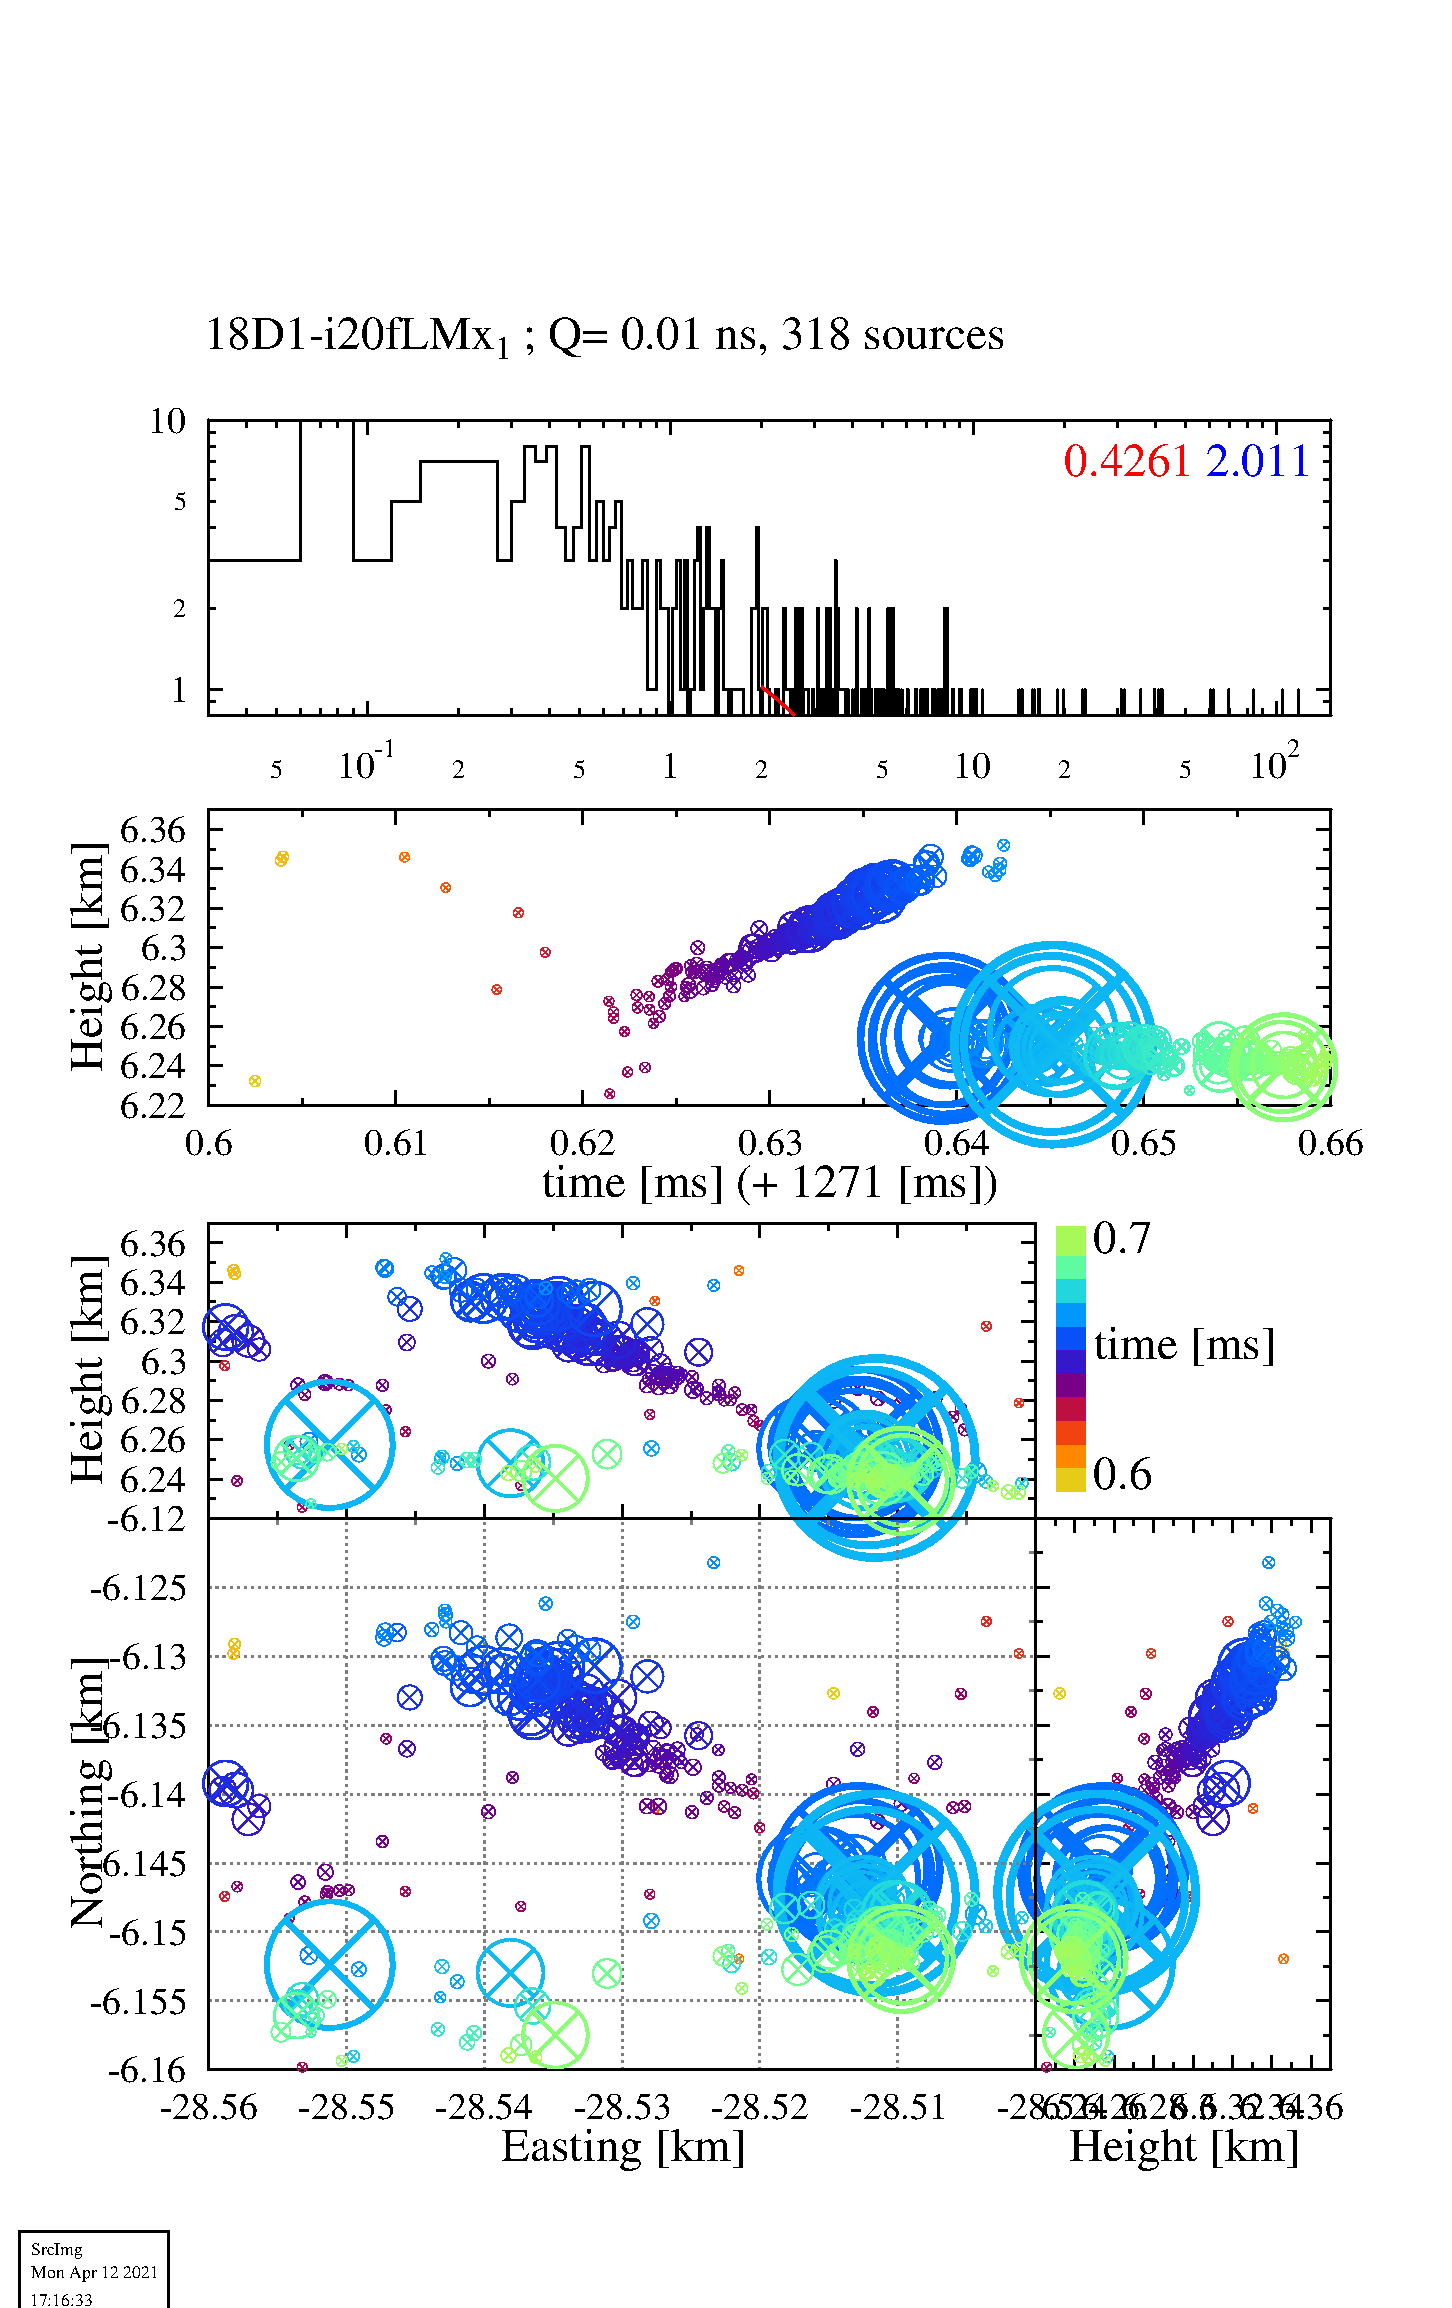
\includegraphics[width=0.49\textwidth]{Figs/18D1-i20fMx_1LIntfSpecSel} }
%\centering{\includegraphics[ bb=1.0cm 2.4cm 24.5cm 25.7cm,clip, width=0.49\textwidth]{../Figs/SE20A7-NPMx_1HIntfSpecSel} }
	\caption{Typical image for the TRID Imager as created by running ``InterfSrcSel.sh".}	 \figlab{TRIDSelSrcsImg}
\end{figure}

The plots will be made for the `Mx' and `Bar' files as well as for X- and Y-dipoles, all resembling \figref{TRIDSelSrcsImg}. This allows for appending seamless the results of different interferometry runs.

